
\documentclass[a4paper]{article}
\usepackage{graphicx}
\usepackage{tikz}
\usepackage{url}
\usetikzlibrary{arrows}

\newcommand{\rospackage}[1]{\textbf{\textit{#1}}}
\begin{document}

\title{Implementation of 2d navigation for a moving base using ROS}
\date{November 2014}
\author{Windel Bouwman}

\maketitle

\tableofcontents

\section{Introduction}

This document describes how the problem of 2d-navigation was solved on a real robot.
The goal of navigation is to safely move a robot from a to b. The robot used
was moving base, the x80sv.

\section{Navigation overview}

The task of navigation can be split up into the following tasks (see also figure \ref{fig:overview}):

\begin{itemize}
  \item Robot control. This task is concerned with controlling the seperate wheels of the robot. Typically this is done using PID control or something alike.
  \item Odometry calculation. By keeping track of wheel motions, the robot position can be
calculated. This method is subjective to drift.
  \item Position and mapping, also known as SLAM, is the task of determining location of the robot in the world, and at the same time reconstructing the world.
  \item Global planning is the task of determining a path through a known map. This requires a search like A* or something like that.
  \item Local planning takes as input the global path and generated the appropriate motion commands for the robot control. It is some sort of setpoint generator. This layer is also responsible for obstacles. When an obstacle is observed, the path may be adjusted.
  \item Semantic interpretation is the process of converting a task into a sequence of locations to be reached. For example the conversion of the sentence "fetch beer" into a path from the current location to nearest fridge.
\end{itemize}

\begin{figure}
  \centering

% Usage of the ticks package:
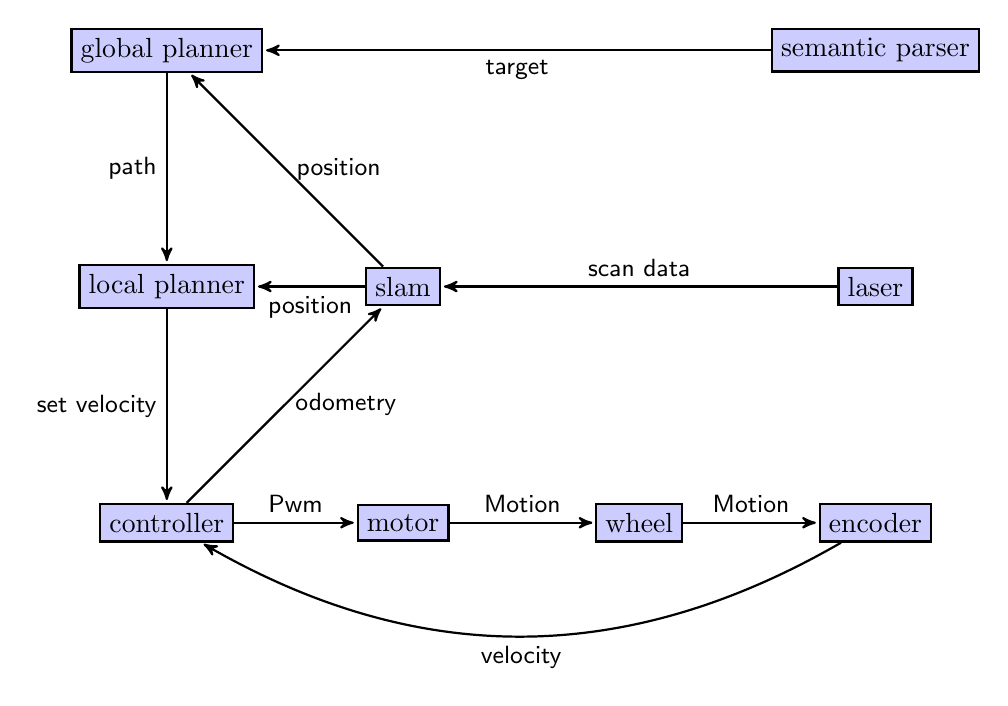
\begin{tikzpicture}[->,>=stealth',shorten >=1pt,auto,node distance=3cm,
  thick,main node/.style={rectangle,fill=blue!20,draw}]

  \node[main node] (1) {controller};
  \node[main node] (2) [right of=1] {motor};
  \node[main node] (3) [right of=2] {wheel};
  \node[main node] (4) [right of=3] {encoder};
  \node[main node] (5) [above of=1] {local planner};
  \node[main node] (7) [right of=5] {slam};
  \node[main node] (6) [above of=5] {global planner};
  \node[main node] (8) [above of=4] {laser};
  \node[main node] (9) [above of=8] {semantic parser};

  \path[every node/.style={font=\sffamily\small}]
    (1)
        edge node [above] {Pwm} (2)
    (2) 
        edge node [above] {Motion} (3)
    (3) 
        edge node[above] {Motion} (4)
    (4) 
        edge [bend left] node [below] {velocity} (1)
    (5) edge node [left] {set velocity} (1)
    (6) edge node [left] {path} (5)
    (7) edge node [right] {position} (6)
    (7) edge node [below] {position} (5)
    (1) edge node [right] {odometry} (7)
    (8) edge node [above] {scan data} (7)
    (9) edge node [below] {target} (6)
    ;
\end{tikzpicture}
  \caption{Subjects involved in the task of navigation}
  \label{fig:overview}
\end{figure}


The rest of this document describes all the tasks listed above as applied to the x80sv using the robot operating system (ROS).

\clearpage

\section{Robot setup}
The robot used in this setup is the x80sv of drrobot. This robot has three wheels, of which
two are controlled. Other sensors are range sensors, infrared and ultrasonic.
The robot is extended with a laser range
sensor (LRS) and a laptop with ROS installed. The LRS and the controllerboard of the x80sv are
connected via usb-serial cables. The controllerboard of the x80sv is provided with
the robot.

\begin{figure}[h!]
  \centering
  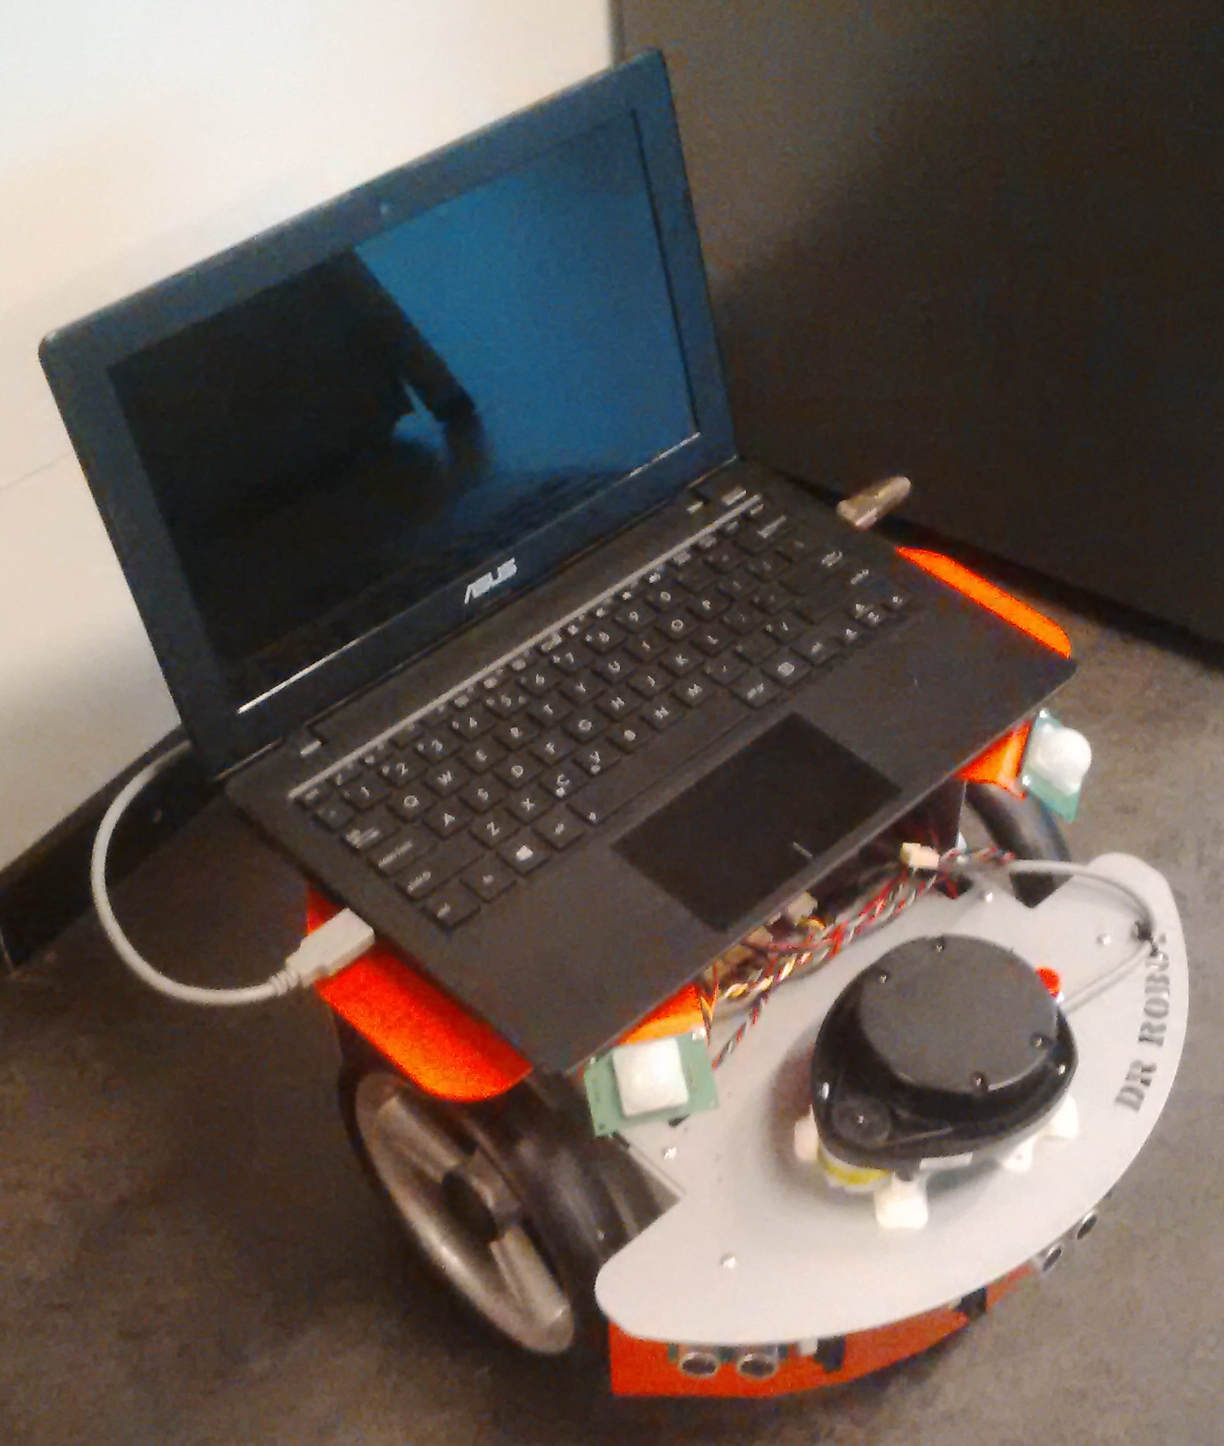
\includegraphics[width=\textwidth,height=\textheight,keepaspectratio]{img/fotorobot.png}
  \caption{Photo of the x80sv equiped with laptop and LRS}
\end{figure}

\subsection{Installation}

To use the robot, install ROS indigo on ubuntu 14.04 on the robot laptop. Download the 
x80sv software from the github repository (\url{https://github.com/saxionled/x80sv}). Follow 
instruction in the readme.

\subsection{Kinematics}

Two-wheeled vehicles have the following kinematic equations of motion:

TODO


\subsection{Control}

The velocity control is done by the controllerboard of the robot. The commands to
the controllerboard are wheel velocities in encoder ticks. A conversion from linear
and angular velocities to wheel velocities is required.

\begin{equation}
        v_{left} = (2 * v_{linear} - v_{angular} * wheelDistance) / (2 * wheelRadius)
\end{equation}
\begin{equation}
        v_{right} = (v_{angular} * wheelDistance + 2 * v_{linear}) / (2 * wheelRadius)
\end{equation}

In the next step, the wheel velocities are translated into encoder velocities.

\begin{equation}
  leftWheelCmd = -motorDir * v_{left} * encoderOneCircleCnt / (2 \pi)
\end{equation}
\begin{equation}
 rightWheelCmd = motorDir * v_{right} * encoderOneCircleCnt / (2 \pi)
\end{equation}

These equations are implemented in the real robot drivers (\url{https://github.com/SaxionLED/x80sv/tree/master/x80sv_driver}). In case of simulation, these equations are done by gazebo.

\subsection{Odometry}
The task of the odometry system is to keep track of the robot position using wheel encoder
data. To implement this for a two wheeled robot the following formulas are used:

\begin{equation}
 d_{left} = calculateMovementDelta(mtr0)
\end{equation}
\begin{equation}
 d_{right} = calculateMovementDelta(mtr1)
\end{equation}
\begin{equation}
 averageDistance = (d_{left} + d_{right}) / 2
\end{equation}
\begin{equation}
 \delta \theta = atan2((d_{right} - d_{left}), wheelDis_);
\end{equation}
\begin{equation}
 \delta x = averageDistance * cos(\theta);
\end{equation}
\begin{equation}
 \delta y = averageDistance * sin(\theta);
\end{equation}
\begin{equation}
 \theta += \delta \theta
\end{equation}
\begin{equation}
 x += \delta x
\end{equation}
\begin{equation}
 y += \delta y
\end{equation}

These equations are implemented in the real robot drivers (\url{https://github.com/SaxionLED/x80sv/tree/master/x80sv_driver}). In case of simulation, these equations are done by gazebo.

\subsection{robot description}
To use the robot with the ROS system, an urdf model must be created. The model of the x80sv is
located in the folder \url{x80sv_description}. The xacro macro system is used to simplify the
writing of the urdf file. The urdf description contains a description of what links and joints
the robot consists of. The model is used by rviz for visualization and by gazebo to construct
the physical model of the robot to simulate it. The weights, shapes and materials of the links
are also specified in this file.

\section{ROS concepts}
\subsection{rviz}
Rviz is an indispensible tool when debugging a robotic system. With rviz one can visualize a robot
and its environment. The tool consists of a main window and a pane to the left where various data
visualizers can be added.

\subsection{rqt}
Another helpful tool when debugging a ros system is rqt. This tool is a plugin container where plugins
can be selected. Plugins exists for tf tree visualization, node interconnect, topic inspection,
logging viewer, diagnostics viewer and more.

\subsection{tf}
The tf (\url{http://wiki.ros.org/tf}) system of ROS is used to describe the various parts of 
a robot in space. The TF-tree of a robot is the relative position of all bodies of a robot
with respect to eachother.

\section{Slam}
Simultaneous localization and mapping (SLAM), is a required component for navigation.
The gmapping node was used in the case of the x80sv.

\subsection{gmapping}

For slam the standard package \rospackage{ros-indigo-gmapping} [1] can be used. 

[1] http://wiki.ros.org/gmapping

This node takes as input the odometry data from the control layer and the laser scan
data. It then is capable of generating a map and determining the drift that occurred
since odometry start.

\subsection{Laser orientation}
The orientation of the laser is important for the gmapping node. The node assumes that
scan is symmetric around zero angle. This means that a laserscan message with range
0 to 2 pi will not work. A range from -pi to pi will work!

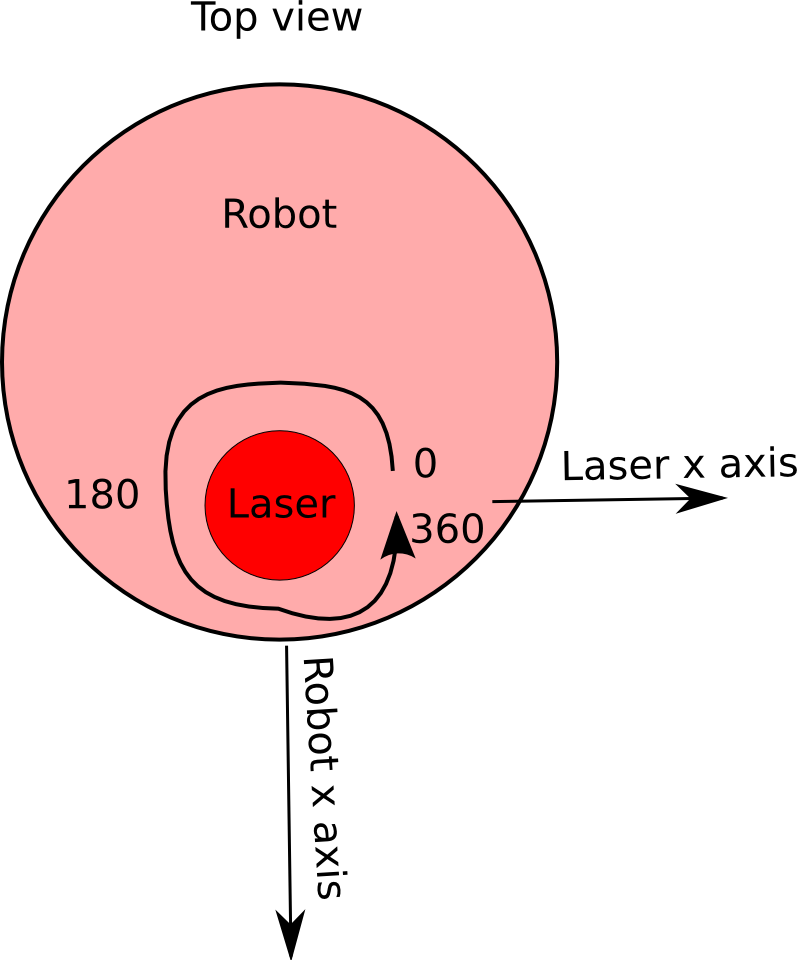
\includegraphics[width=0.5\textwidth,height=\textheight,keepaspectratio]{img/laser_orientation.png}

\section{Simulation}
Instead of trying to run everything on the real robot, a simulated version of the x80sv
was created. This was done using the gazebo simulator. Gazebo is a physics simulator, which can be
used with ROS.

With this simulation it is possible to run the exact same navigation software with the real
robot as well as with the simulated variant.

\begin{figure}[h!]
  \centering
  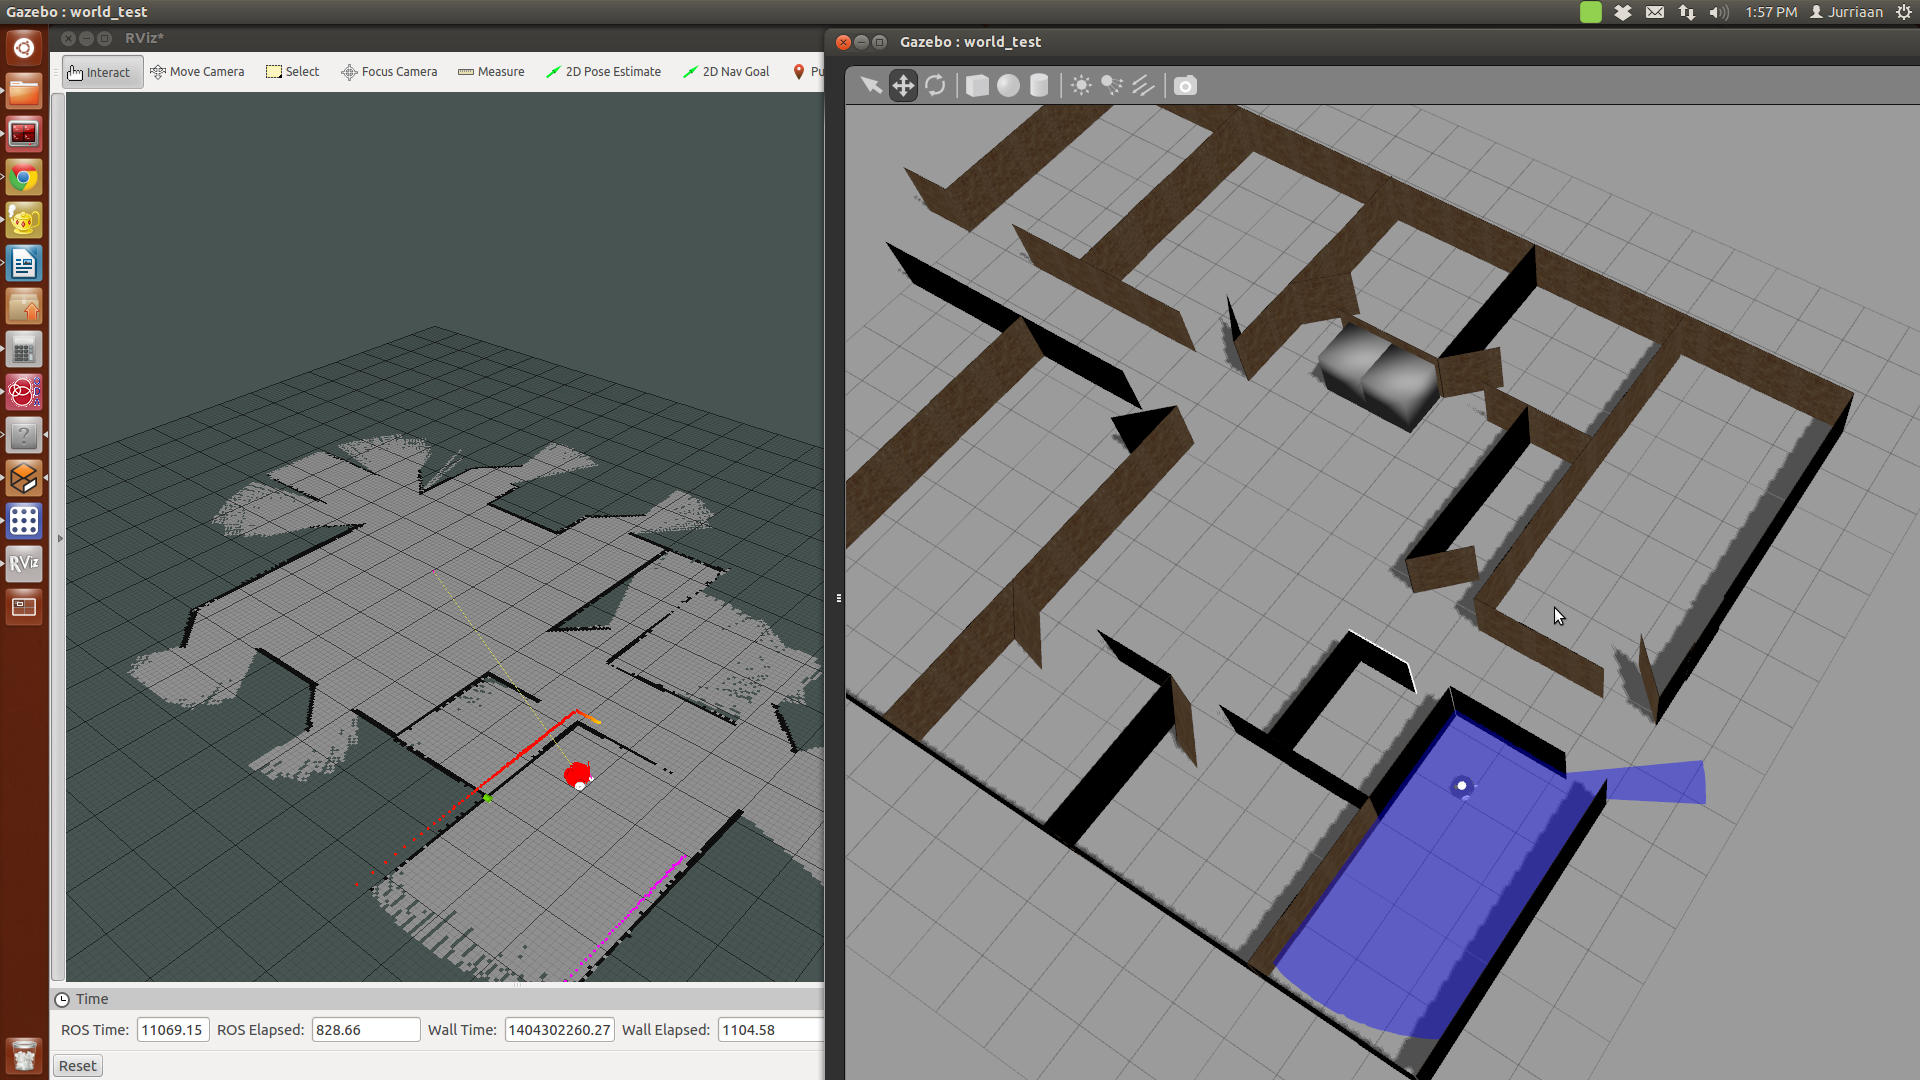
\includegraphics[width=\textwidth,height=\textheight,keepaspectratio]{img/office_sim_testgmapping.png}
  \caption{Gazebo (right) and rviz (left) running a simulated robot}
\end{figure}

\begin{figure}[h!]
  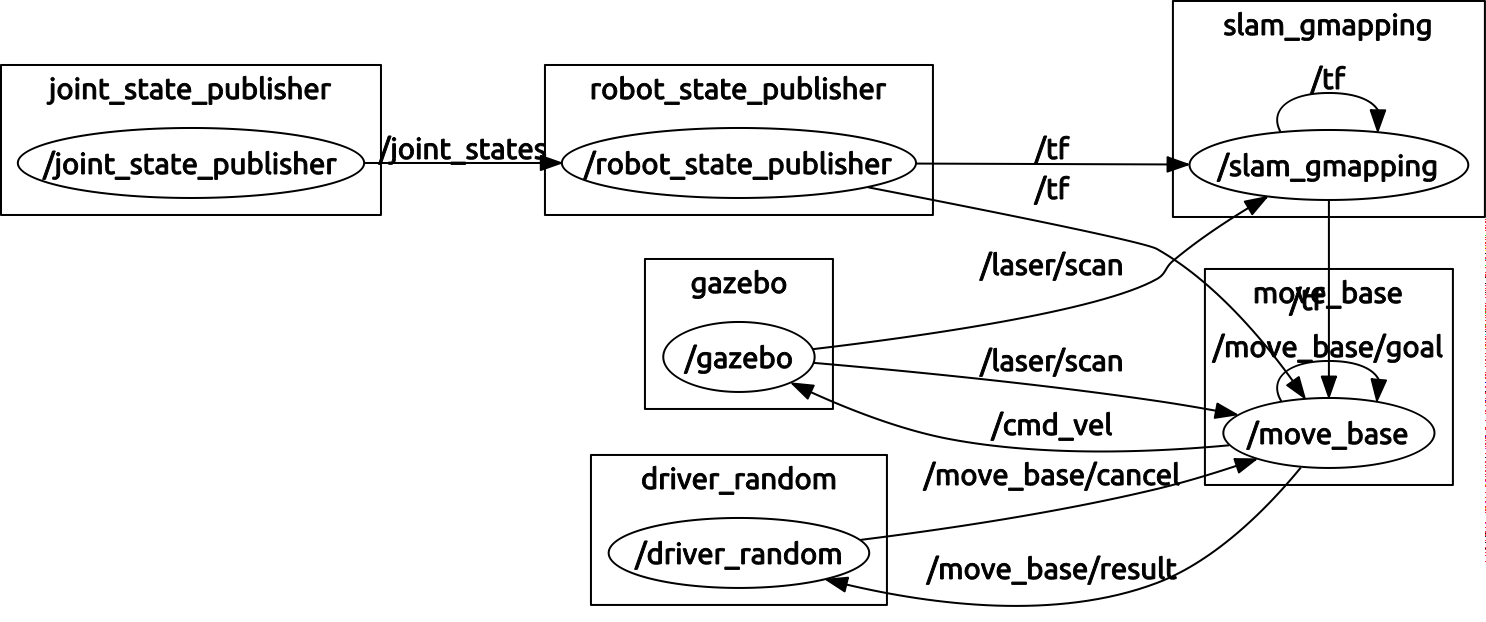
\includegraphics[width=\textwidth,height=\textheight,keepaspectratio]{img/simulatie_nodes.png}
  \caption{The nodes involved in the simulation}
\end{figure}

\section{Navigation}

\subsection{Framework}

There is an existing framework for 2d mobile base navigation \url{http://wiki.ros.org/move_base}.
Another framework is the skynav framework developed at saxion \url{https://github.com/SaxionLED/skynav}

\subsection{skynav}
TODO

\subsection{move base}

The \rospackage{ros-indigo-move-base} package provides a sort of infrastructure for 2d mobile base
navigation. It provides a structure into which plugins can be inserted.
Among plugins are costmap function, recovery behaviors, local planner and global planner.

\begin{figure}[h!]
  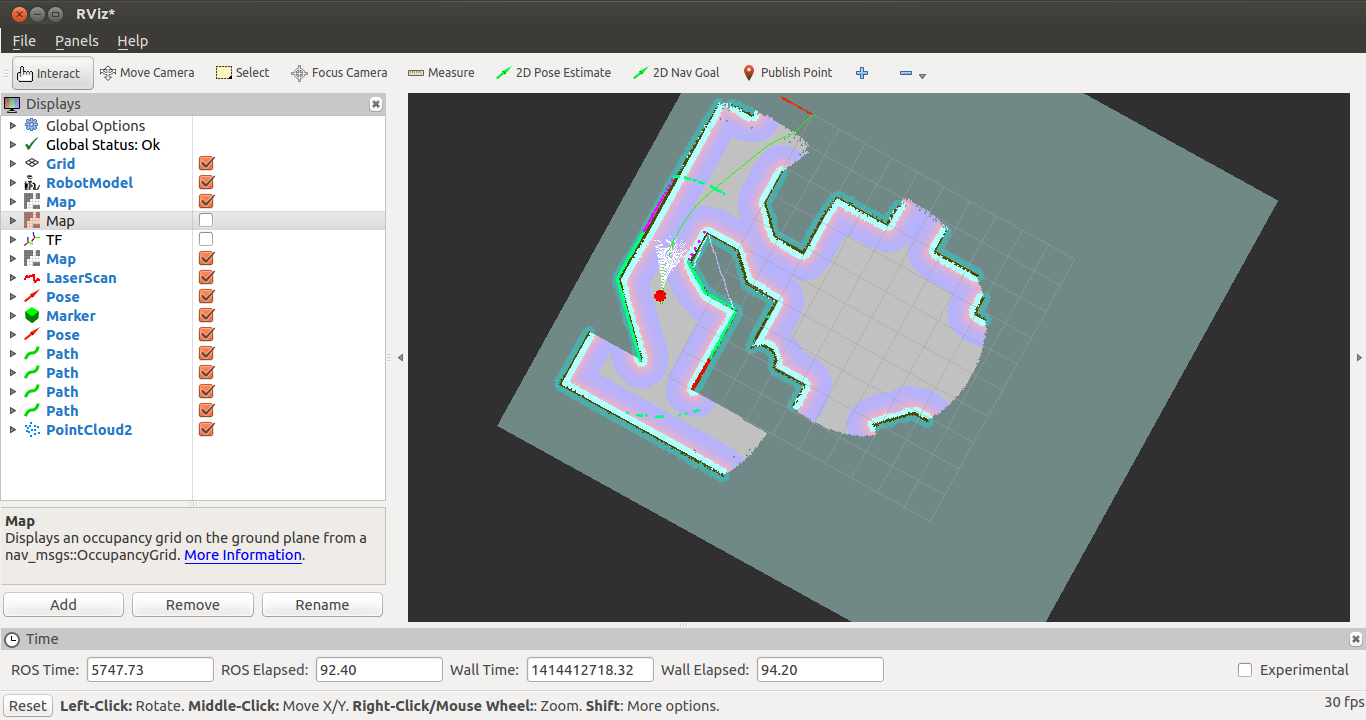
\includegraphics[width=\textwidth,height=\textheight,keepaspectratio]{img/rviz_navigation2.png}
  \caption{Navigation visualized in rviz}
  \label{fig:navrviz}
\end{figure}

\subsection{costmap2d}
The \rospackage{ros-indigo-costmap-2d} is a ros package that can create a costmap of the environment
of the robot.
The costmap is then used by both global and local planning to determine the path.
The costmap consists of several input layers. The static layer takes the map as determined by
gmapping and inflates it somehwat. The obstacle layer can incorporate different sensors.
Rviz can be used to visualize these costmaps.

\section{Global planning}

\subsection{global planner}
The \rospackage{ros-indigo-global-planner} package contains a global planner that uses simple search
for an optimal path given a costmap. It is a plugin for use with move-base.

\subsection{navfn planner}
The \rospackage{ros-indigo-navfn} package provides another plugin for move-base for global navigation.

\subsection{move-base-ompl}
This package contains a plugin wrapper for ompl. Ompl is a motion planning library using random trees.
Random trees follow the idea of randomly exploding a tree of all possible state of a robot
given its current position and vehicle dynamics.

\url{https://github.com/windelbouwman/move-base-ompl}

\url{http://ompl.kavrakilab.org/}

\section{Local planning}

\subsection{base local planner}

The default planner of the move base package for ROS is the base local planner.
This planner uses dynamic window approach (DWA) to plan a path. This means that from the current 
location several path options are simulated in advance and the one with the least cost is selected.

This planner has several parameters that must be tuned.

\subsection{DWA local planner}
The dwa local planner is also a standard ROS planner. It is contained in the package
\rospackage{ros-indigo-dwa-local-planner}.

\subsection{Smooth planner}
The smooth planner is own work, and is located at github (
\url{https://github.com/SaxionLED/x80sv/tree/master/smooth_local_planner}).
This planner follow the global path and when confronted with an obstacle simply
reports that the plan has failed and waits for new commands from the global planner.

\section{Future work}

\begin{itemize}
  \item The skynav navigation stack could be transformed to work via the plugin system of move base ros package.
\end{itemize}

\end{document}

